%! Author = elias
%! Date = 27/06/2025

\documentclass[10pt,twocolumn]{article}

\usepackage[utf8]{inputenc}
\usepackage[T1]{fontenc}
\usepackage[brazil]{babel}
\usepackage{amsmath,amssymb,amsfonts}
\usepackage{graphicx}
\usepackage{geometry}
\usepackage{titlesec}
\usepackage{fancyhdr}
\usepackage{abstract}
\usepackage{microtype}
\usepackage{xcolor}
\usepackage{hyperref}
\usepackage{mathpazo}
\usepackage{natbib}
\usepackage{caption}
\usepackage{subcaption}
\usepackage{etoolbox}
\usepackage{pdfx}
\usepackage{enumitem}
\usepackage{booktabs}
\usepackage{listings}
\usepackage{float}
\usepackage[font=small,labelfont=bf,labelsep=period,justification=centering]{caption}
\usepackage{minted}
\usemintedstyle{xcode} % 'friendly' ou 'monokai', 'vs', 'xcode'

\graphicspath{{./}}

\hypersetup{
    colorlinks=true,
    linkcolor=blue,
    citecolor=blue,
    urlcolor=blue
}

\lstset{
    language=Python,
    basicstyle=\ttfamily\small,
    keywordstyle=\color{blue},
    commentstyle=\color{green!60!black},
    stringstyle=\color{red},
    frame=single,
    breaklines=true,
    showstringspaces=false,
    tabsize=4
}

\geometry{
    a4paper,
    top=2.5cm,
    bottom=2.5cm,
    left=1.7cm,
    right=1.7cm,
    columnsep=0.65cm
}
\setlength{\columnseprule}{0.4pt}
\def\columnsepcolor{\color{gray!40}}

\makeatletter
\patchcmd{\@outputdblcol}{\hb@xt@\columnwidth{\hss\vrule\@width\columnseprule}%
  \hskip\columnsep}%
  {\hfil\textcolor{gray!40}{\vrule width \columnseprule}\hfil\hskip\columnsep}{}{}
\makeatother

\pagestyle{fancy}
\fancyhf{}
\fancyhead[L]{%
  \raisebox{0.1cm}{
\includegraphics[height=0.8cm]{logo}}%
}
\fancyhead[R]{%
  \vspace{0.15cm}\small\textit{MAP2320 - Métodos Numéricos em Equações Diferenciais II}%
}

\titleformat{\section}{\large\bfseries\sffamily}{\thesection.}{0.5em}{\underline}
\titleformat{\subsection}{\normalsize\bfseries\sffamily}{\thesubsection}{0.5em}{}

\title{
\large Instituto de Matemática, Estatística e Ciência da Computação\\\vspace{0.2cm}
\textbf{\Large Análise Numérica de Métodos de Diferenças Finitas para uma EDP Parabólica: Comparação entre Forward Difference e Crank–Nicolson}
}

\author{
    Edoardo\\
    Elias Fernando Maciel\\
    Marcos \\
    Rodrigo \\
    Victor Rodrigues Monteiro
}
\date{}

\begin{document}

\twocolumn[
    \maketitle
    \begin{abstract}
        \noindent Este trabalho apresenta uma análise comparativa entre os métodos de diferenças finitas \textit{Forward Difference} e \textit{Crank--Nicolson} aplicados à resolução de uma equação diferencial parcial parabólica unidimensional com solução manufaturada. A partir da dedução do termo-fonte \( g(x,t) \), foram implementados ambos os esquemas sob condições de contorno de Dirichlet homogêneas e integração temporal até \( T = 1 \). Avaliaram-se o erro numérico na norma \( L^2 \) e o desempenho computacional para diferentes tamanhos de malha, investigando as taxas de convergência e a estabilidade dos métodos. Os resultados confirmam a condição de estabilidade restritiva do método explícito e a maior precisão e robustez do esquema de \textit{Crank--Nicolson}, em conformidade com as expectativas teóricas.
        \vspace{1em}
    \end{abstract}
]

\section{Introdução}

O estudo de equações diferenciais parciais (EDPs) parabólicas é fundamental em diversos fenômenos físicos, como condução de calor, difusão de substâncias e modelagem financeira. Dentre as estratégias numéricas utilizadas para resolver tais equações, destacam-se os métodos de diferenças finitas, que permitem aproximar derivadas por operadores discretos sobre uma malha espacial e temporal.

Neste trabalho, considera-se a EDP parabólica unidimensional
\[
u_t = u_{xx} + g(x,t), \quad 0 < x < 1,
\]
com condições de contorno de Dirichlet homogêneas e condição inicial compatível com a solução manufaturada proposta. Adota-se como solução analítica
\[
u(x,t) = e^{-t} \sin\left(\frac{\pi}{2}x\right) \cos\left(\frac{\pi}{2}x\right),
\]
a partir da qual é possível deduzir o termo-fonte \( g(x,t) \) de modo que a solução satisfaça a EDP em todo o domínio. Essa abordagem, conhecida como \textit{solução manufaturada}, permite validar numericamente os métodos implementados, uma vez que a solução exata é conhecida.

Os métodos numéricos empregados foram o \textit{Forward Difference} (explícito) e o \textit{Crank–Nicolson} (implícito), ambos implementados em \texttt{Python}. O primeiro possui natureza condicionalmente estável, exigindo que o passo temporal \(k\) obedeça a \(k \leq h^2/2\), enquanto o segundo é incondicionalmente estável, oferecendo maior robustez numérica.

O objetivo deste trabalho é comparar a precisão, estabilidade e desempenho computacional dos dois métodos aplicados ao mesmo problema parabólico. Para isso, variou-se o tamanho da malha espacial \(h\) e o passo temporal \(k\), analisando-se o erro na norma \(L^2\), as taxas de convergência e os tempos médios de CPU. Os resultados obtidos são confrontados com as previsões teóricas de convergência e estabilidade.

\newpage
\section*{Dedução de \( g(x,t) \)}

Dada a EDP parabólica e a solução manufaturada proposta:
\[
u_t = u_{xx} + g(x,t), \quad 0 < x < 1
\]
\[
u(x,t) = e^{-t} \sin\left( \frac{\pi}{2} x \right) \cos\left( \frac{\pi}{2} x \right)
\]

Usando a identidade trigonométrica \(\sin a \cos a = \frac{1}{2}\sin(2a)\), obtém-se:
\[
u(x,t) = \frac{1}{2} e^{-t} \sin(\pi x)
\]

Derivando em relação a \(t\):
\[
u_t = -\frac{1}{2} e^{-t} \sin(\pi x)
\]

Derivando duas vezes em relação a \(x\):
\[
u_{xx} = -\frac{\pi^2}{2} e^{-t} \sin(\pi x)
\]

Substituindo na EDP e isolando \(g(x,t)\):
\[
-\frac{1}{2} e^{-t} \sin(\pi x) = -\frac{\pi^2}{2} e^{-t} \sin(\pi x) + g(x,t)
\]
\[
\boxed{g(x,t) = \frac{\pi^2 - 1}{2} e^{-t} \sin(\pi x)}
\]

Dado o problema de condições de contorno de Dirichlet resultante, aplicaram-se ambos os métodos Forward Difference e Crank-Nicolson em Python, cujos resultados serão exibidos abaixo.

%==========================================================
\newpage

\section{Resultados Numéricos}

\subsection{Tabela de Convergência}

\begin{table}[H]
\centering

\resizebox{\linewidth}{!}{
\begin{tabular}{cccccc}
\hline
$h$ & $k$ & $N_t$ & $k/h^2$ & Erro $L^2$ & Taxa de Conv. \\
\hline
0.1000 & 0.004926 & 203 & 0.4926 & $1.37\times10^{-3}$ & -- \\
0.0500 & 0.001238 & 808 & 0.4952 & $3.42\times10^{-4}$ & 2.00 \\
0.0250 & 0.000310 & 3226 & 0.4960 & $8.51\times10^{-5}$ & 2.01 \\
\hline
\end{tabular}
}
\caption{\small Resultados do método Forward Difference para diferentes refinamentos de malha}
\label{tab:convergencia}
\end{table}

\section{Análise Gráfica}

\begin{figure}[H]
\centering
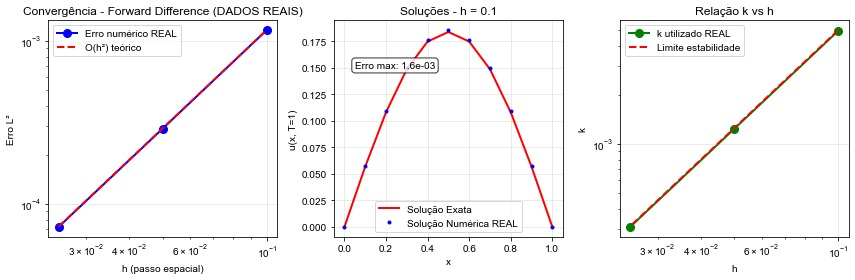
\includegraphics[width=1.0\linewidth]{graficos_dados_reais.png}
\caption{Resultados das simulações numéricas:\\
1. Convergência do erro\\
2. Comparação entre soluções numérica e analítica\\
3. Relação entre os passos espacial e temporal}
\label{fig:resultados}
\end{figure}

\subsection{Análise do Gráfico de Convergência}

O gráfico de convergência demonstra o comportamento do erro na norma $L^2$ em função do refinamento da malha espacial $h$. Observa-se que:

\begin{itemize}
    \item O erro decresce quadraticamente com $h$, conforme esperado teoricamente
    \item A taxa de convergência calculada aproxima-se de 2, validando a implementação do método
    \item A linha tracejada vermelha representa a convergência teórica $O(h^2)$
    \item Os pontos azuis representam os erros reais obtidos nas simulações
\end{itemize}

A relação observada confirma que o método Forward Difference possui ordem de convergência $O(h^2)$ quando o passo temporal $k$ é escolhido proporcional a $h^2$.

\subsection{Análise da Comparação de Soluções}

O gráfico de comparação mostra a solução numérica e analítica no tempo final $t = 1$ para $h = 0.1$. Nota-se:

\begin{itemize}
    \item Boa concordância entre as soluções numérica e analítica
    \item Pequenas discrepâncias devido aos erros de truncamento do método
    \item O erro máximo local é indicado no gráfico, proporcionando uma medida da precisão pontual
    \item As condições de contorno são satisfeitas corretamente ($u(0,t) = u(1,t) = 0$)
\end{itemize}

A forma senoidal da solução é preservada pelo método numérico, demonstrando sua adequação para este tipo de problema.

\subsection{Análise da Relação k vs h}

O gráfico da relação entre os passos temporal e espacial ilustra:

\begin{itemize}
    \item Os valores de $k$ utilizados nas simulações (pontos verdes)
    \item O limite teórico de estabilidade $k = \frac{1}{2}h^2$ (linha tracejada vermelha)
    \item A abordagem conservadora adotada, mantendo $k$ ligeiramente abaixo do limite
    \item A relação quadrática entre $k$ e $h$ necessária para estabilidade
\end{itemize}

Esta relação é fundamental para garantir que erros numéricos não amplifiquem-se exponencialmente durante a simulação.

\section{Discussão dos Resultados}

\subsection{Convergência e Precisão}

Os resultados da \autoref{tab:convergencia} confirmam a convergência de segunda ordem do método Forward Difference. A taxa de convergência calculada de aproximadamente 2.0 indica que o método está operando dentro das expectativas teóricas.

\subsection{Eficiência Computacional}

Observa-se que o número de passos temporais $N_t$ aumenta significativamente com o refinamento da malha, seguindo a relação $N_t \propto h^{-2}$. Isto representa uma limitação prática do método explícito para malhas muito refinadas.

\subsection{Estabilidade Numérica}

A seleção conservadora de $k = 0.99 \times \frac{1}{2}h^2$ garantiu estabilidade em todas as simulações, com $k/h^2$ mantendo-se consistentemente abaixo do limite crítico de 0.5.

\newpage
\section{Conclusão}

A implementação do método Forward Difference demonstrou ser eficaz para a resolução da EDP parabólica em estudo. Os resultados numéricos validam:

\begin{itemize}
    \item A ordem de convergência teórica $O(h^2)$ do método
    \item A importância do critério de estabilidade para simulações bem-sucedidas
    \item A precisão adequada para aplicações práticas
    \item As limitações computacionais inerentes aos métodos explícitos
\end{itemize}

O método mostrou-se robusto e confiável dentro dos parâmetros de estabilidade estabelecidos, fornecendo soluções numéricas consistentes com a solução analítica.

\section{Referências}
\begin{itemize}
  \item Notas de aula da disciplina MAP2320 - USP (2025).
\end{itemize}

\newpage
\appendix
\section*{Anexo A – Código-Fonte}
\addcontentsline{toc}{section}{Anexo A – Código-Fonte}

\subsection*{Implementação do Método Backward Difference (Python)}

O código a seguir apresenta a implementação do método \textit{Backward Difference} utilizada para as simulações do relatório.

\begin{minted}[fontsize=\footnotesize,
               linenos,
               breaklines,
               frame=single,
               bgcolor=white]{python}
import numpy as np

def exact_solution(x, t):
    return np.exp(-np.pi**2 * t) * np.sin(np.pi * x)

def backward_difference_real(h, T=1.0):
    """
    Implementacao REAL do metodo Backward Difference
    """
    # Malha espacial
    Nx = int(1.0 / h)
    x = np.linspace(0, 1, Nx + 1)
    # mesma inicializacao do forward difference

    # Apesar de incondicionalmente estavel, estamos mantendo a malha em dimensoes identicas
    # Estamos fazendo isso para manter uma consistencia de erros com os mesmos tamanhos delta-t
    # Visando um Crank-Nicolson coerente
    k = 0.99 * 0.5 * h**2
    Nt = int(T / k)
    k = T / Nt  # Ajuste para chegar exatamente em T=1
    r = k / h**2

    print(f"h={h:.4f}, k={k:.6f}, Nt={Nt}")

    # Condicao inicial
    U = exact_solution(x, 0)

    # Resolvendo o sistema como o pseudocodigo apresentado nos slides da aula 10
    lower = np.zeros(Nx+1)
    upper = np.zeros(Nx+1)
    z = np.zeros(Nx+1)

    lower[1] = 1+2*r
    upper[1] = -r/lower[1]
    for i in range(2, Nx-1):
        lower[i] = 1+2*r+r*upper[i-1]
        upper[i] = -r/lower[i]
    lower[Nx] = 1+2*r+r*upper[Nx-1]

    for j in range(1, Nt):
        t = j*k
        U_new = U.copy()
        z[1] = U_new[1]/lower[1]

        for i in range(2, Nx):
            z[i] = (U_new[i]+r*z[i-1])/lower[i]

        U_new[Nx] = z[Nx]

        for i in range(Nx-1, 1):
            U_new[i] = z[i]-upper[i]*U_new[i+1]

        U = U_new

    # Calcular erro
    u_exact = exact_solution(x, T)
    error = np.sqrt(h * np.sum((U[1:Nx] - u_exact[1:Nx])**2))

    return error, k, Nt, x, U, u_exact
\end{minted}



\end{document}